\begin{itemize}
  \item Contact-rich manipulation tasks require haptic and visual feedback
  \item Use self-supervision to learn multimodal representation of inputs that are used to improve sample efficiency for policy learning
  \item Evaluated method on peg insertion for different geometry, configurations, and clearances
  \item Contact-rich tasks: peg insertation, block packing, edge following
  \item Diverse set of modalities including vision, range, audio, haptic, proprioceptive data and language and often these are complementary of each other
  \item DL usually requires lot of high-dimensional training data and self-supervision does not rely on having human annotated data
  \item Their model encodes 3 types of data: RGB, haptic feedback from F/T sensor, and proprioceptive data from joint encoders
  \item Heterogenuous nature requires domain-specific encoders for each modality
  \item Generate labels automatically through self-supervision
  \item The model has to predict 1) the optical flow generated by action and 2) whether end-effector will make contact with environment
  \item To exploit concurrency between data streams, use a third objective that predicts whether two streams are temporally aligned (binary classification)
  \begin{figure}[H]
    \caption{Multimodal fusion model}
    \centering
    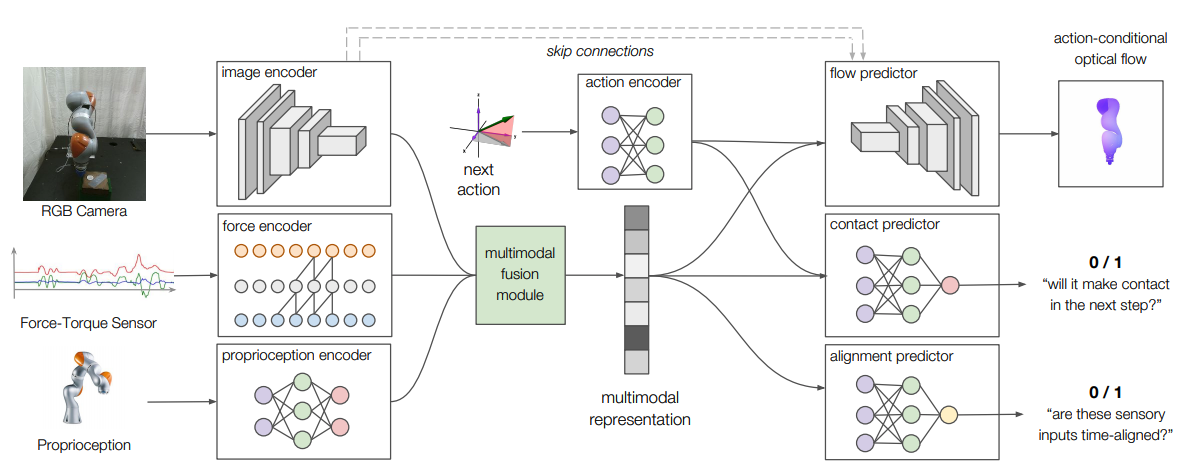
\includegraphics[width=\textwidth]{../../imgs/multimodal_contact_tasks.png}
  \end{figure}
  \begin{figure}[H]
    \caption{Controller}
    \centering
    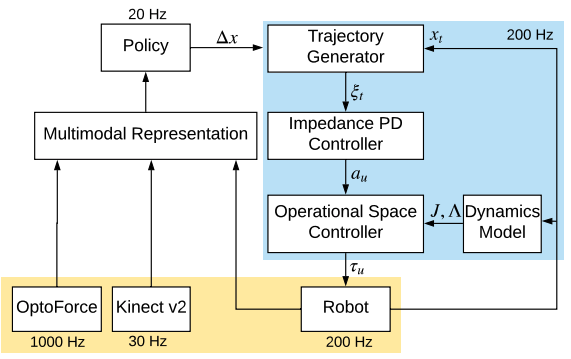
\includegraphics[width=0.5\textwidth]{../../imgs/contact_controller.png}
  \end{figure}
  \item Model-free removes need for an accurate dynamics model (hard to obtain in presence of rich contacts), use TRPO for policy learning
  \item Policy network is 2-layer MLP that takes in 128-d multimodal rep and produces a 3D displacementof end-effector
  \item Policy outputs Cartesian-control commands instead of joint-space commands
  \item Use direct torque control because it gives robot compliance making it safer
  \item Also make use of a staged-reward function for subtasks to simplify the challenge of exploration
  \item Conduct ablation study to learn about importance of each modality, also study robustness of policy in presence of sensor noise and external perturbation (e.g. pushing robot arm)
  \item Lots of other challenges in real-world: sensor synchronization, variable delays, real-world dynamics, etc
\end{itemize}